\subsection{Гравитационное линзирование}

\textit{Гравитационная линза} --- массивное тело или система тел (галактик, скопление галактик, скопление тёмной материи), искривляющая своим гравитационным полем направление распространения электромагнитного излучения.

На (Рис.\ref{grav-lens}) показано, как происходит гравитационное линзирование. S --- источник электромагнитных волн, O --- наблюдатель, $J_1$ и $J_2$ --- видимые положения источника, $M$ --- массивное тело.

\begin{figure}[h!]
\begin{center}
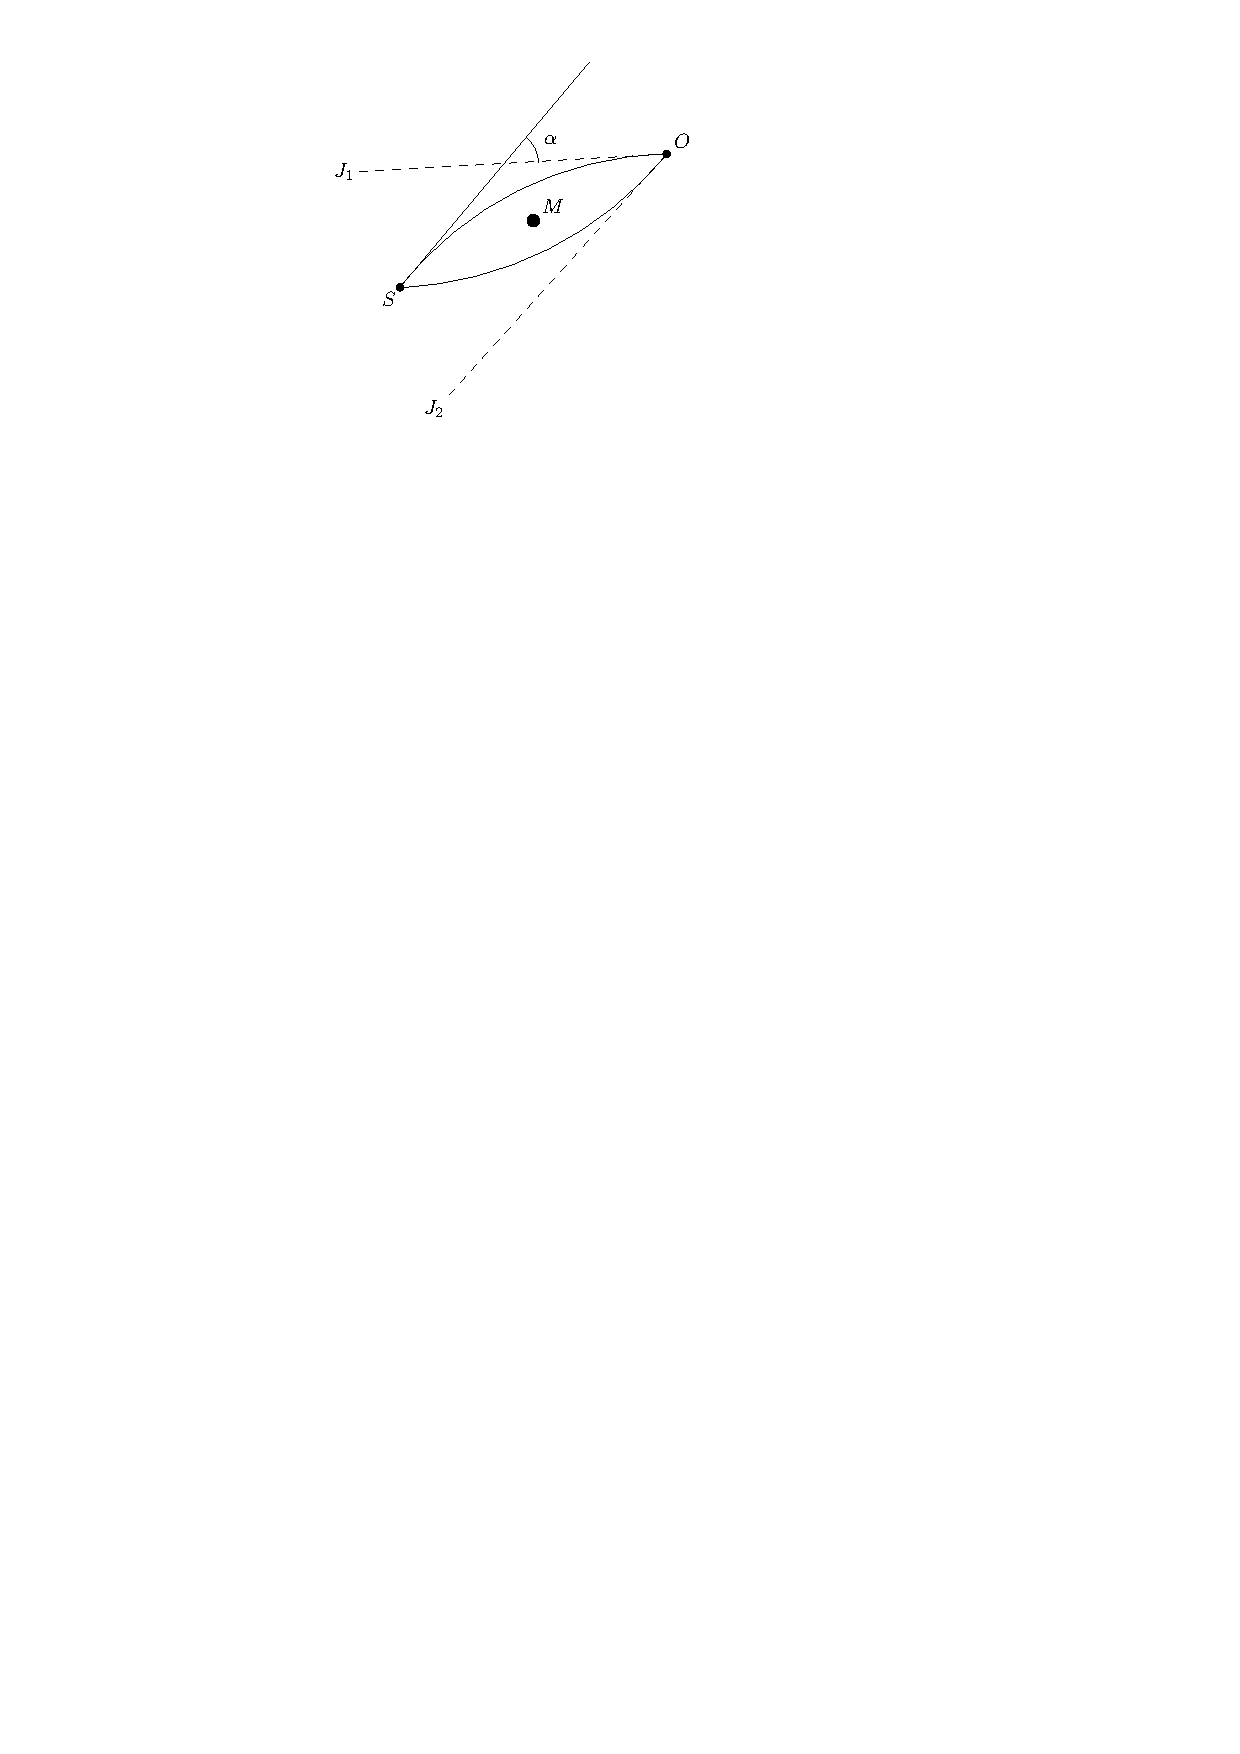
\includegraphics[width=0.4\textwidth]{grav-lens}
\caption{Гравитационное линзирование}\label{grav-lens}
\end{center}
\end{figure}

Найти угол отклонения луча в радианах можно по следующей формуле:
\begin{equation}
\alpha=\frac{4GM}{Rc^2},
\end{equation}
где $M$ --- масса тела, отклоняющего луч, $R$ --- радиус этого тела, $c$ --- скорость света.